\chapter{Model}
\label{Model}


A model has been made with two goal of answering two questions:
\begin{enumerate}\itemsep2pt
	\item How strong are the reflections of flashes in a realistic environment?
	\item How much will these reflections change if an object enters the illuminated area
\end{enumerate}
This section describes how the model explained in section \ref{sec:Characteristics of light} was adjusted and implemented to answer the questions posed above

\section{Model description}
The model made is an interpretation of the phong reflection model (see section \ref{sec:Characteristics of light}). It calculates how much of the light leaving a luminaire, bounces back via the environment to a photodiode placed next to the light source. This section will first discuss the adjustments made to the phong model, followed by an explanation of the calculation process.

\subsection{Adjustments}
The first adjustment is the removal of "time". The methods in the literature took the travelling time of light into account in order to calculate the possible inter-symbol interference. This is not required for this simulation as we are only interested in the steady state situation when the light is fully turned on and the light received by the photodiode is maximized for the current situation.

The second adjustment is the removal of "colour". The original method differentiated between different wavelengths of visible light when reflecting light of off surfaces and was therefore maintaining colour information. This is however not necessary for this model, as we do not care about the colour of the reflecting objects, but only about the total amount of energy reflected by the object. For this reason, the surface reflection coefficient ($p(\lambda)$) was replaced with the albedo of the object instead.

Albedo is a property of an object representing the percentage of energy which is reflected when sun is shining on the object. Even though albedo is based on the full spectrum of sunlight instead of only the wavelengths of visible light, it gives a reasonable approximation of the reflection coefficient in this scenario. This will be shown in section \ref{sec:verification}.

\begin{equation}
\Gamma = \int_{380nm}^{780nm} \Phi_e p(\lambda) d\lambda \to \Gamma = \Phi_{lum} \alpha
\end{equation}

The final adjustment is the amount of reflections we calculate. In reality a light ray can be reflected an infinite amount of times of several different surfaces before returning back to the sensor. In the model however we only calculated one bounce (from the light to an object and back) for two reasons. The reason for this is that the first reflection provides approximately 80\% of the signal where all other reflections only make up 20\% of the total power\cite{indoor_VLC_no_LOS}. This increase in accuracy

\begin{equation}
\label{eq:Ehor_new}
E_{hor}=\frac{I(\phi)\cos(\varphi)}{d^2}=\frac{I(0) cos^m(\phi)\cos(\varphi)}{d^2}
\end{equation}

\subsection{Calculation process}
Calculating the amount of light reflecting back to the object is a three step process. The first step is to calculate the shadow casted by the object on the floor and walls. This is required as the surface where the shadow is casted can't reflect light back directly to the photo diode. It's important to note that light casting the shadow is reflected of the object instead and with that, changes the reflection pattern of the room.

The second step is to calculate how much light reflected from all floors and walls (where no shadow is casted) to the photo diode. The finals step is to calculate how much light is reflected from each side of the object. \ref{fig:raytracing} shows an overview of an environment with rays leaving the light, casting shadow and the resulting reflections.

\begin{figure}
	\centering     %%% not \center
	\label{fig:raytracing}
	\subfigure[Sideview]{\label{fig:a}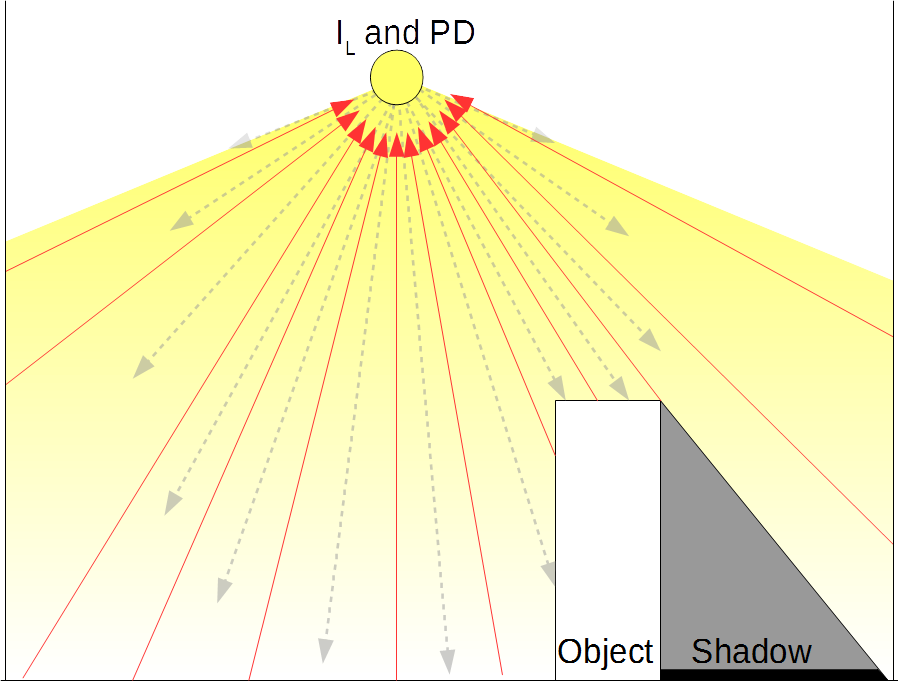
\includegraphics[width=68mm]{pics/Calculation_frontview.png}}
	\subfigure[Topview]{\label{fig:b}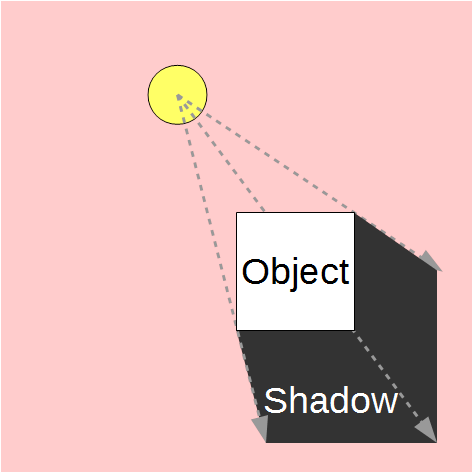
\includegraphics[width=52mm]{pics/Calulation_topview.png}}
	\caption{Overview of the calculation process. Grey lines represent light rays casted by the light. Black represents the shadow casted by the object on the floor or walls. Red lines or areas show reflections bouncing from the ground, walls or object back to the photo diode.}
\end{figure}

\section{Verification}
\label{sec:verification}
The calculation method was verified using a scale model featuring a LED\cite{lamptest}, a paper box and a light meter\cite{LuxMeter}. The first step of verifying the model is check if the LED is modelled properly. This was done by hanging the LED at 100cm above the floor and measuring the horizontal illuminance ($E_hor$) at the floor to see if the measured irradiation pattern of the LED matches the theoretical pattern produced by equation \ref{eq:I(phi)}. Simulations in Appendix \ref{app_repository} that the LED in the test set-up was producing more light than in the specification.

The second step is the verification of the interpretation of the Phong model. This was done with the test set-up shown in figure \ref{fig:VerificationSetup}. By moving a paper box across the flool in steps of 5cm and measuring the reflection at each step we obtain the red line in figure \ref{fig:verf_floor}.

\begin{figure}[]
	\centering
	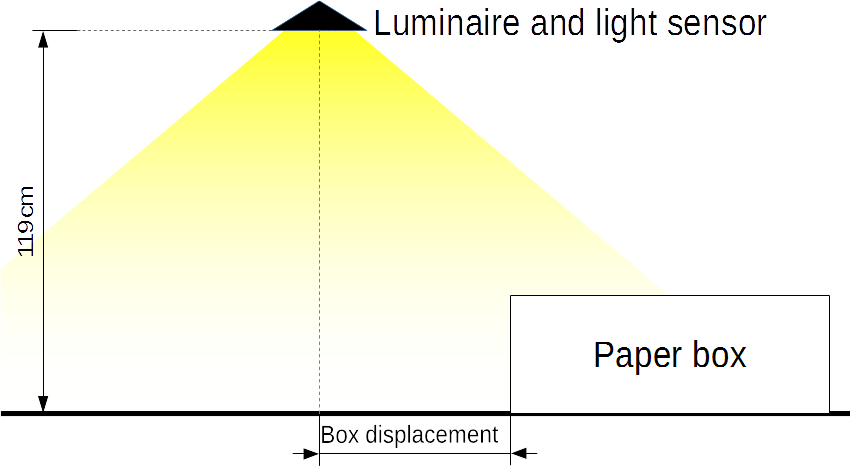
\includegraphics[width=\textwidth]{pics/Verification_Situation.png}
	\caption{Visualisation of the model verification set-up.}
	\label{fig:VerificationSetup}
\end{figure}

\begin{figure}
	\centering     %%% not \center
	\label{fig:VerificationResults}
	\subfigure[]{\label{fig:verf_paper}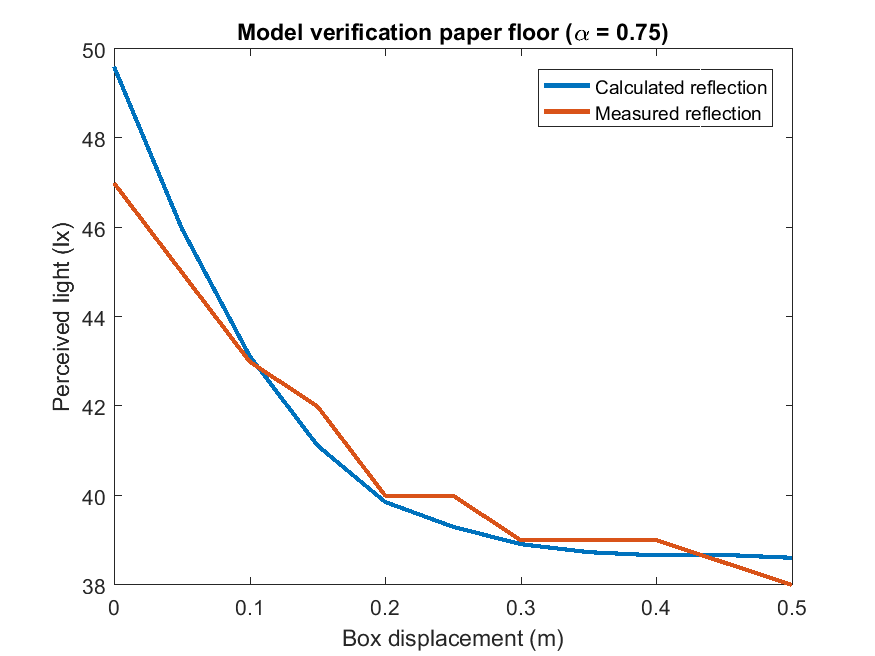
\includegraphics[width=60mm]{pics/ModelVerificationResults_paper.png}}
	\subfigure[]{\label{fig:verf_floor}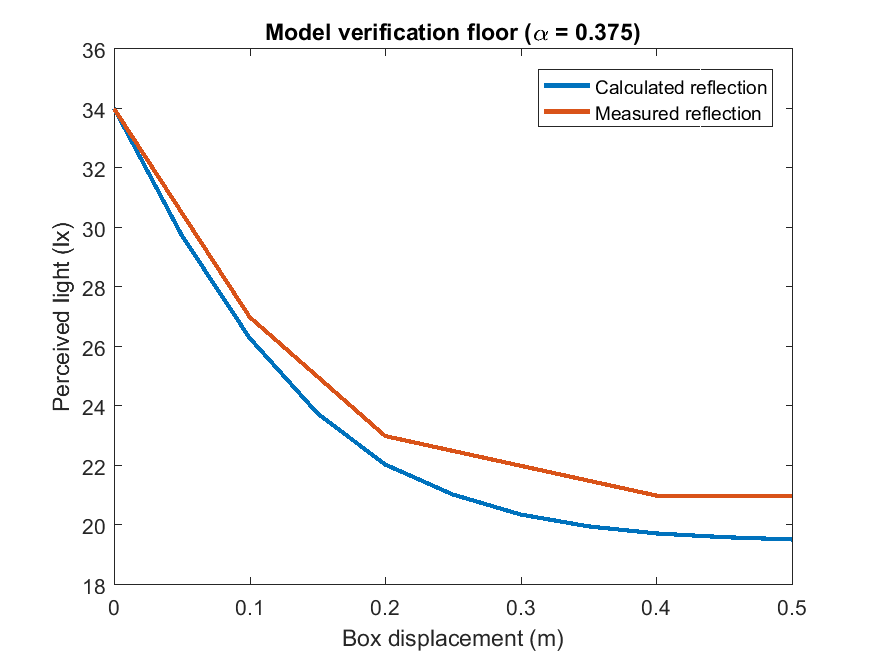
\includegraphics[width=60mm]{pics/ModelVerificationResults_floor.png}}
	\caption{Both figures show that the model provides a reasonable approximation of the reality. Note that the albedo of paper was taken from \cite{Albedo} and the albedo of the floor was estimated with these measurements.}
\end{figure}

\section{Modelling of the hallway}
\label{sec:moddelingofthehallway}
The hallway modelled is based on a real hallway located at the TU Delft. The hallway is 2.2m wide and 2.8m high. The floors albedo is set at 0.37, as this was calculated during the verification of the model. The albedo of the walls was set to 0.95 which represents the albedo of white plaster\cite{Albedo}. The reflection of these surfaces is assumed to be fully diffuse ($r_d = 1$).

Industry standards state that corridors in education buildings should be illuminated with at least $E_{mean} > 100lx$ and a light uniformity of $U_o > 0.4$\cite{lichthandbuch}. These lighting requirements can be achieved using the same luminaire used during the verification process if hung in the staggered formation shown in figure \ref{fig:pattern_hallway}. Calculations showing that the industry standards are met can be found in Appendix \ref{app_repository}.

The object passing by the light (representing a human) will be modelled as a cuboid 0.5m long and 0.2m wide with varying heights. Several albedos have been assigned to the cuboid to represent the different kind of clothing humans wear. The object will be moved in a straight line trough the hallway with the light at a set vertical distance y. Some example paths can be seen in figure \ref{fig:traveling_path}.

\begin{figure}
	\centering     %%% not \center
	\subfigure[Staggerd hallway LED pattern ]{\label{fig:pattern_hallway}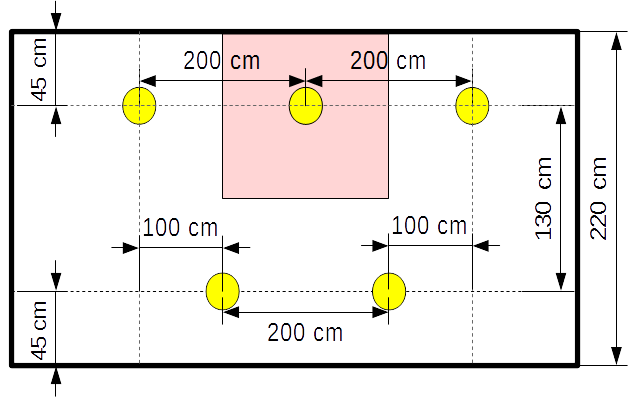
\includegraphics[width=60mm]{pics/LightsOverview.png}}
	\subfigure[Traveling path of the object ]{\label{fig:traveling_path}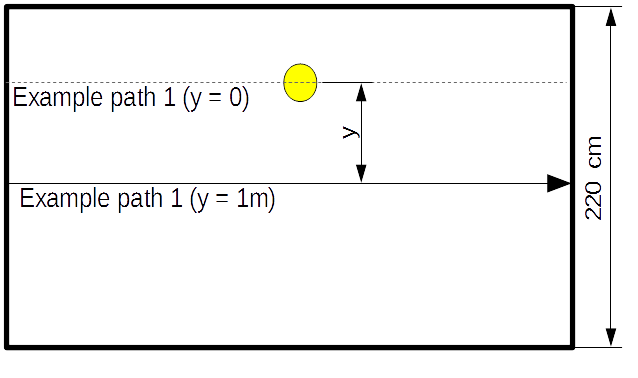
\includegraphics[width=60mm]{pics/TravelingPath.png}}
	\caption{Figure a shows the position of the luminairs to obtain a realistic illumination pattern. Figure b shows an example travelling path of an object.}
\end{figure}

\section{Modelling of the street}
The street model is based on a real street near the TU delft. It has two lanes for a cars (each 3m wide), and sidewalk (2m wide). The albedo of the street will be modeled with different values for old ($\alpha = 0.06$) and new asphalt ($\alpha = 0.14$), as asphalt loses reflectivity if it grows older\cite{Albedo}. The reflections of the street are assumed to be fully diffuse ($r_d = 1$).

Industry standards state that a street with side walk should be illuminated with at least $E_{mean} > 3lx$ and a light uniformity of $U_o > 0.2$ \cite{HandboekBestaandeBouw}.These lighting requirements can be achieved using 700lx luminaires with a halfpower angle of $60^{\circ}$ placed every 15 meter in between the road and side walk. This set-up is visualized in figure \ref{fig:pattern_street}. Calculations showing that the industry standards are met can be found in Appendix \ref{app_repository}.

In this model two different objects will be modelled representing humans (walking on the side walk) and cars (driving in the two driving lanes). The humans will be modelled in the same way as in section \ref{sec:moddelingofthehallway}. The car will be modelled as a cuboid with the dimensions of an Opel Corsa (4m x 1,7m x 1,5m), a commonly seen small car. The object was modelled with diffuse reflection, because no reliable sources describing the specular parameters ($r_d$ and $m$) of cars could be found.

Lacking the specular deflection for this specific model should not influence the results significantly. This is because no part of the car will be moved directly underneath the light and therefore no significant amount of light of the spread reflection should ever reach the light sensor. This is visualized in figure \ref{fig:streetnospecular}. This is also the reason why cars are simulated with lower albedo than humans.

\begin{figure}
	\centering     %%% not \center
	\subfigure[Topview of the street model ]{\label{fig:pattern_street}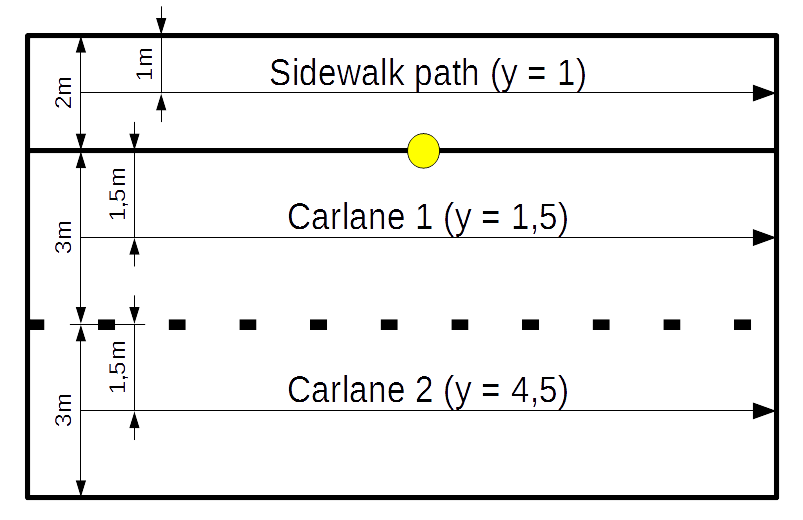
\includegraphics[width=70mm]{pics/TravelingPath_street.png}}
	\subfigure[Spread reflection on cars ]{\label{fig:streetnospecular}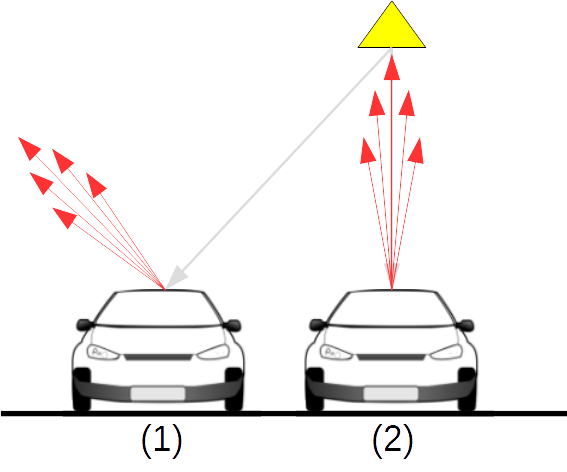
\includegraphics[width=50mm]{pics/StreetNoSpecular.png}}
	\caption{A shows an overview of the model. B shows why the spread reflection component plays no part in this model for cars.}
\end{figure}

\section{Results}
Several measurements have been graphed in Figure X. Raw results can be viewed in appendix \ref{app:RawModelResults}.

%voeg plaatjes toe voor conlusie

\section{Conclusions}

Influence of albedo

approximate the minimum and maximum signal frequency.


